\documentclass{article}
\usepackage[utf8]{inputenc}
\usepackage{hyperref}
\usepackage[letterpaper, portrait, margin=1in]{geometry}
\usepackage{enumitem}
\usepackage{amsmath}
\usepackage{booktabs}
\usepackage{graphicx}

\usepackage{hyperref}
\hypersetup{
colorlinks=true,
    linkcolor=black,
    filecolor=black,      
    urlcolor=blue,
    citecolor=black,
}
\usepackage{natbib}

\usepackage{titlesec}
  
\title{HW6}
\author{Ryan Ellis}
\date{Spring semester 2023}
  
\begin{document}
  
\maketitle

\section{Python}
\subsection{}
\begin{itemize}
    \item Because the policy contains a strict requirement, we expect a sharp RD design. In other words, we do not expect to see cars over the length threshold go \textit{untreated}.
\end{itemize}

\subsection{}
\begin{figure}[!h]
    \centering
    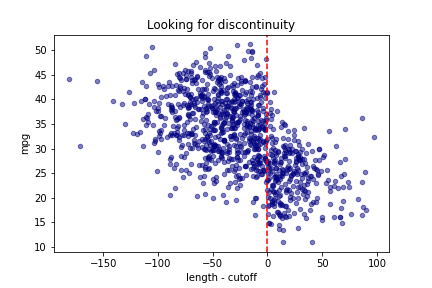
\includegraphics[scale=.9]{homework6/output/scatterplot.png}
    \caption{The discontinuity is not immediately evident from this plot alone. While there are more points near the cutoff than far from it, this is likely because the cutoff itself is fairly near the sample average of lengths (which should be normally distributed in the population). There is little evidence of manipulation of the running variable.}
    \label{fig:my_label}
\end{figure}

\end{document}